I was able to train the agent for the full length of 10 million steps only once, I did a second run with 1 million steps. During the training for each game the score achieved, timesteps taken and final epsilon value where recorded. Achieving a heigher score is the primary goal for this agent. Taking more timesteps means the agent survives longer and has more opportunities to accidentily hit a block and score a poiont. For both training sessions I show the value of epsilon, the score and the timesteps per game vs training progress. For the score and timesteps per game we also plot a moving average created with a window size of 50. We expect score and timesteps per game to be highly correlated. 

\begin{figure}
    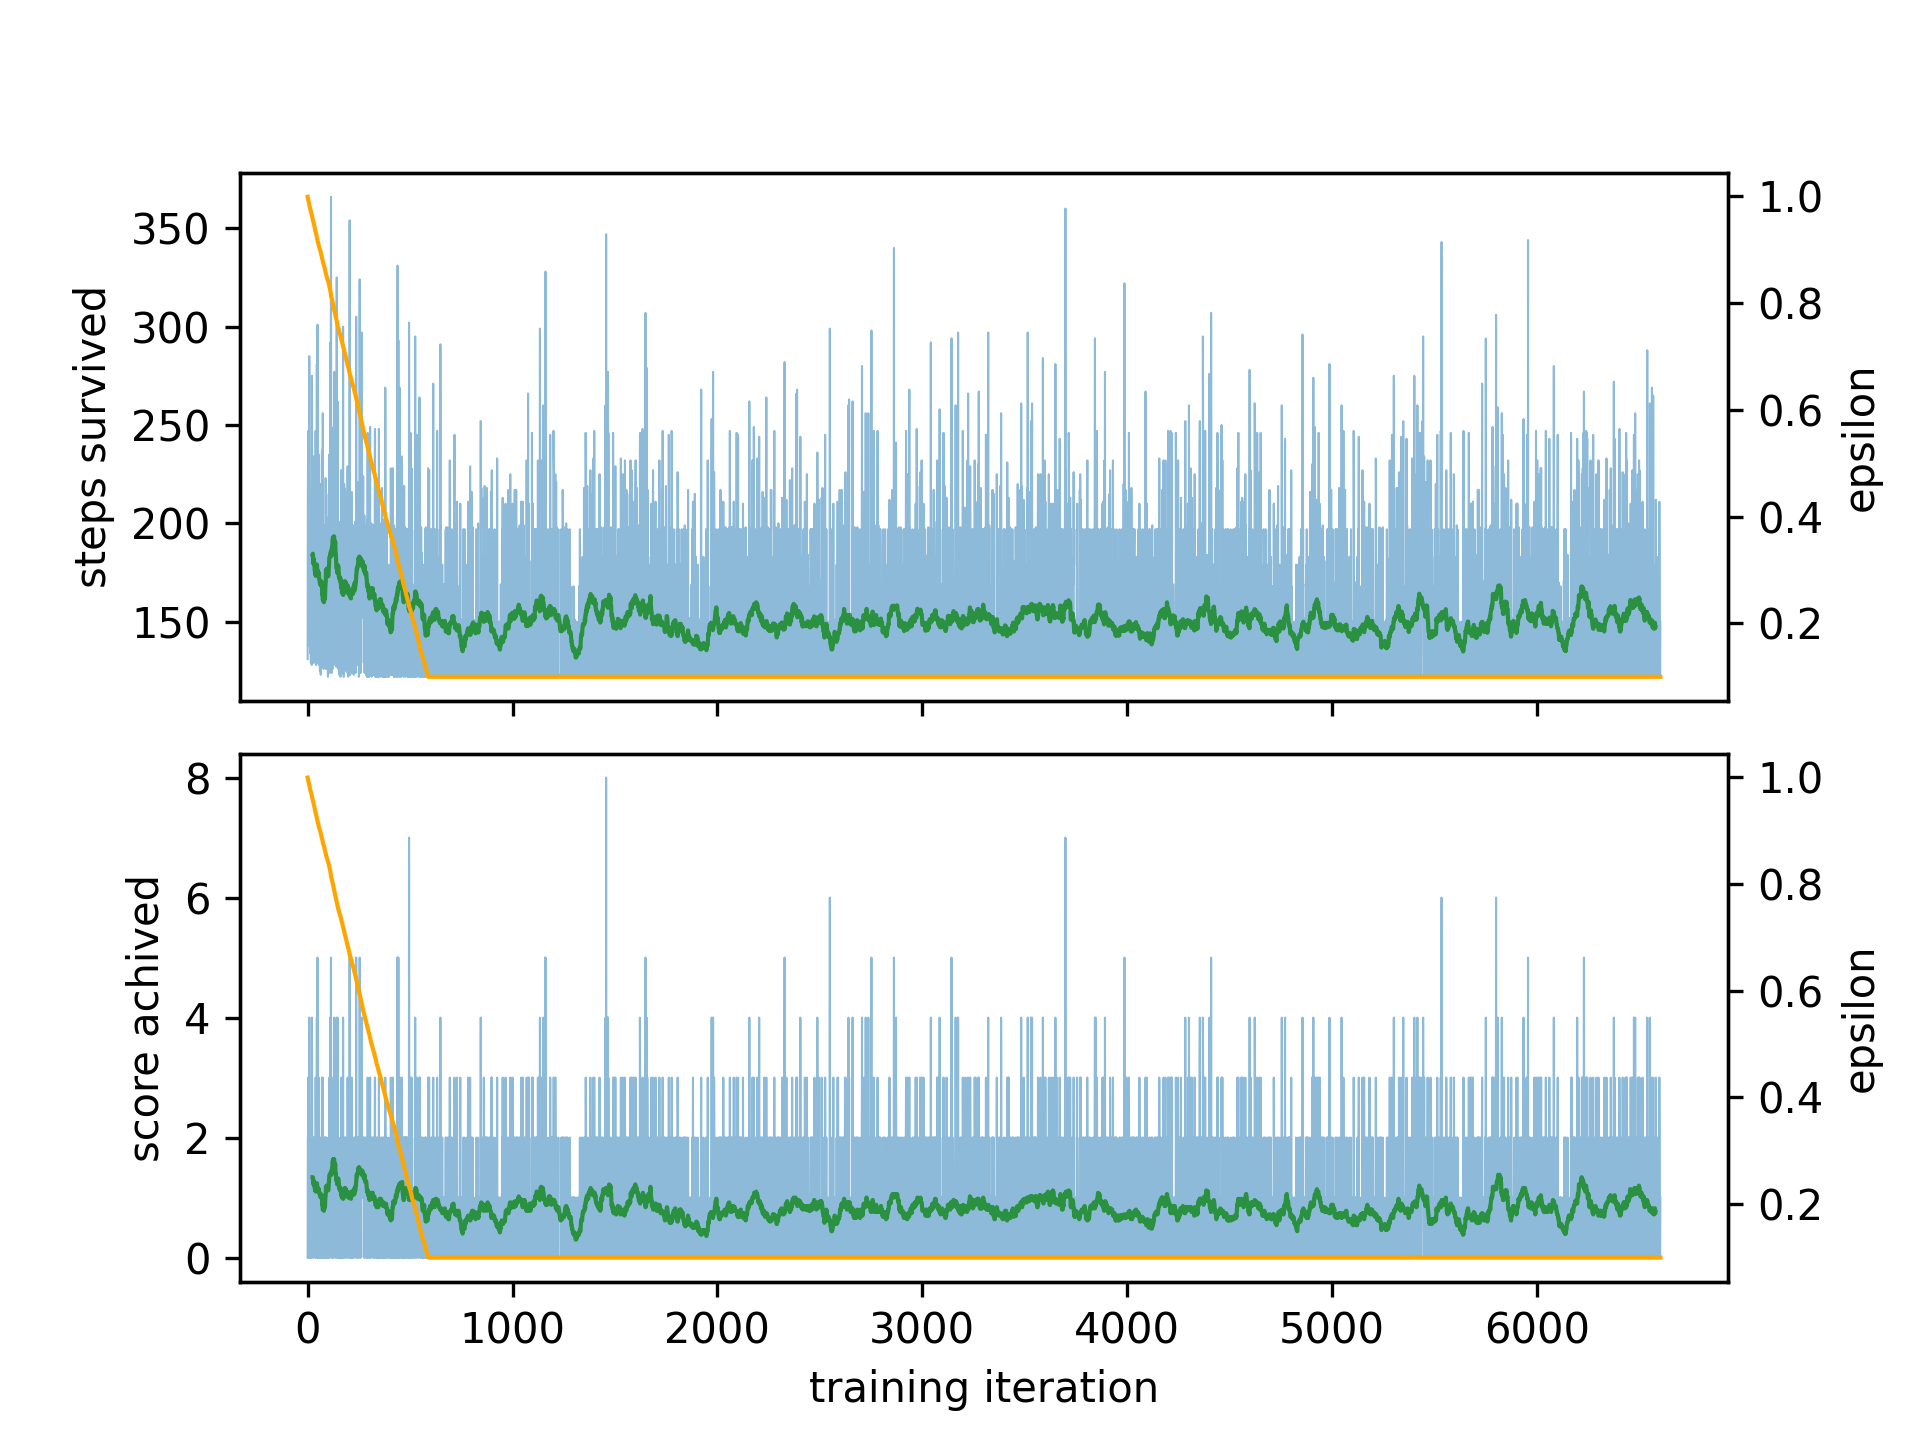
\includegraphics{breakout_1m}
    \caption{The performance of the agent when trained for 1 million steps. In orange the value of epsilon, in blue the steps per game for the top plot and score achived in the bottom plot. In green the moving average over the blue lines.}
    \label{fig:breakout_1m}
\end{figure}

In \autoref{fig:breakout_1m} we see how the agents performans during a training of 1 million steps. The behaviour of the agent is unstable it scores bad during the training not reaching howvering around a score of 1.2 which is the mean score for a random agent\cite{atari}. At around zero the agent seems take longer then later during training, I could not reproduce this thus attribute it to the randomness of the agent, especially as it mostly took random actions here due to the high epsilon value. 

When we train longer for 10 million steps we see a number of hopfull jumps before the agent jumps in performance around game $36000$, see \autoref{fig:breakout_10m}. 

\begin{figure}
    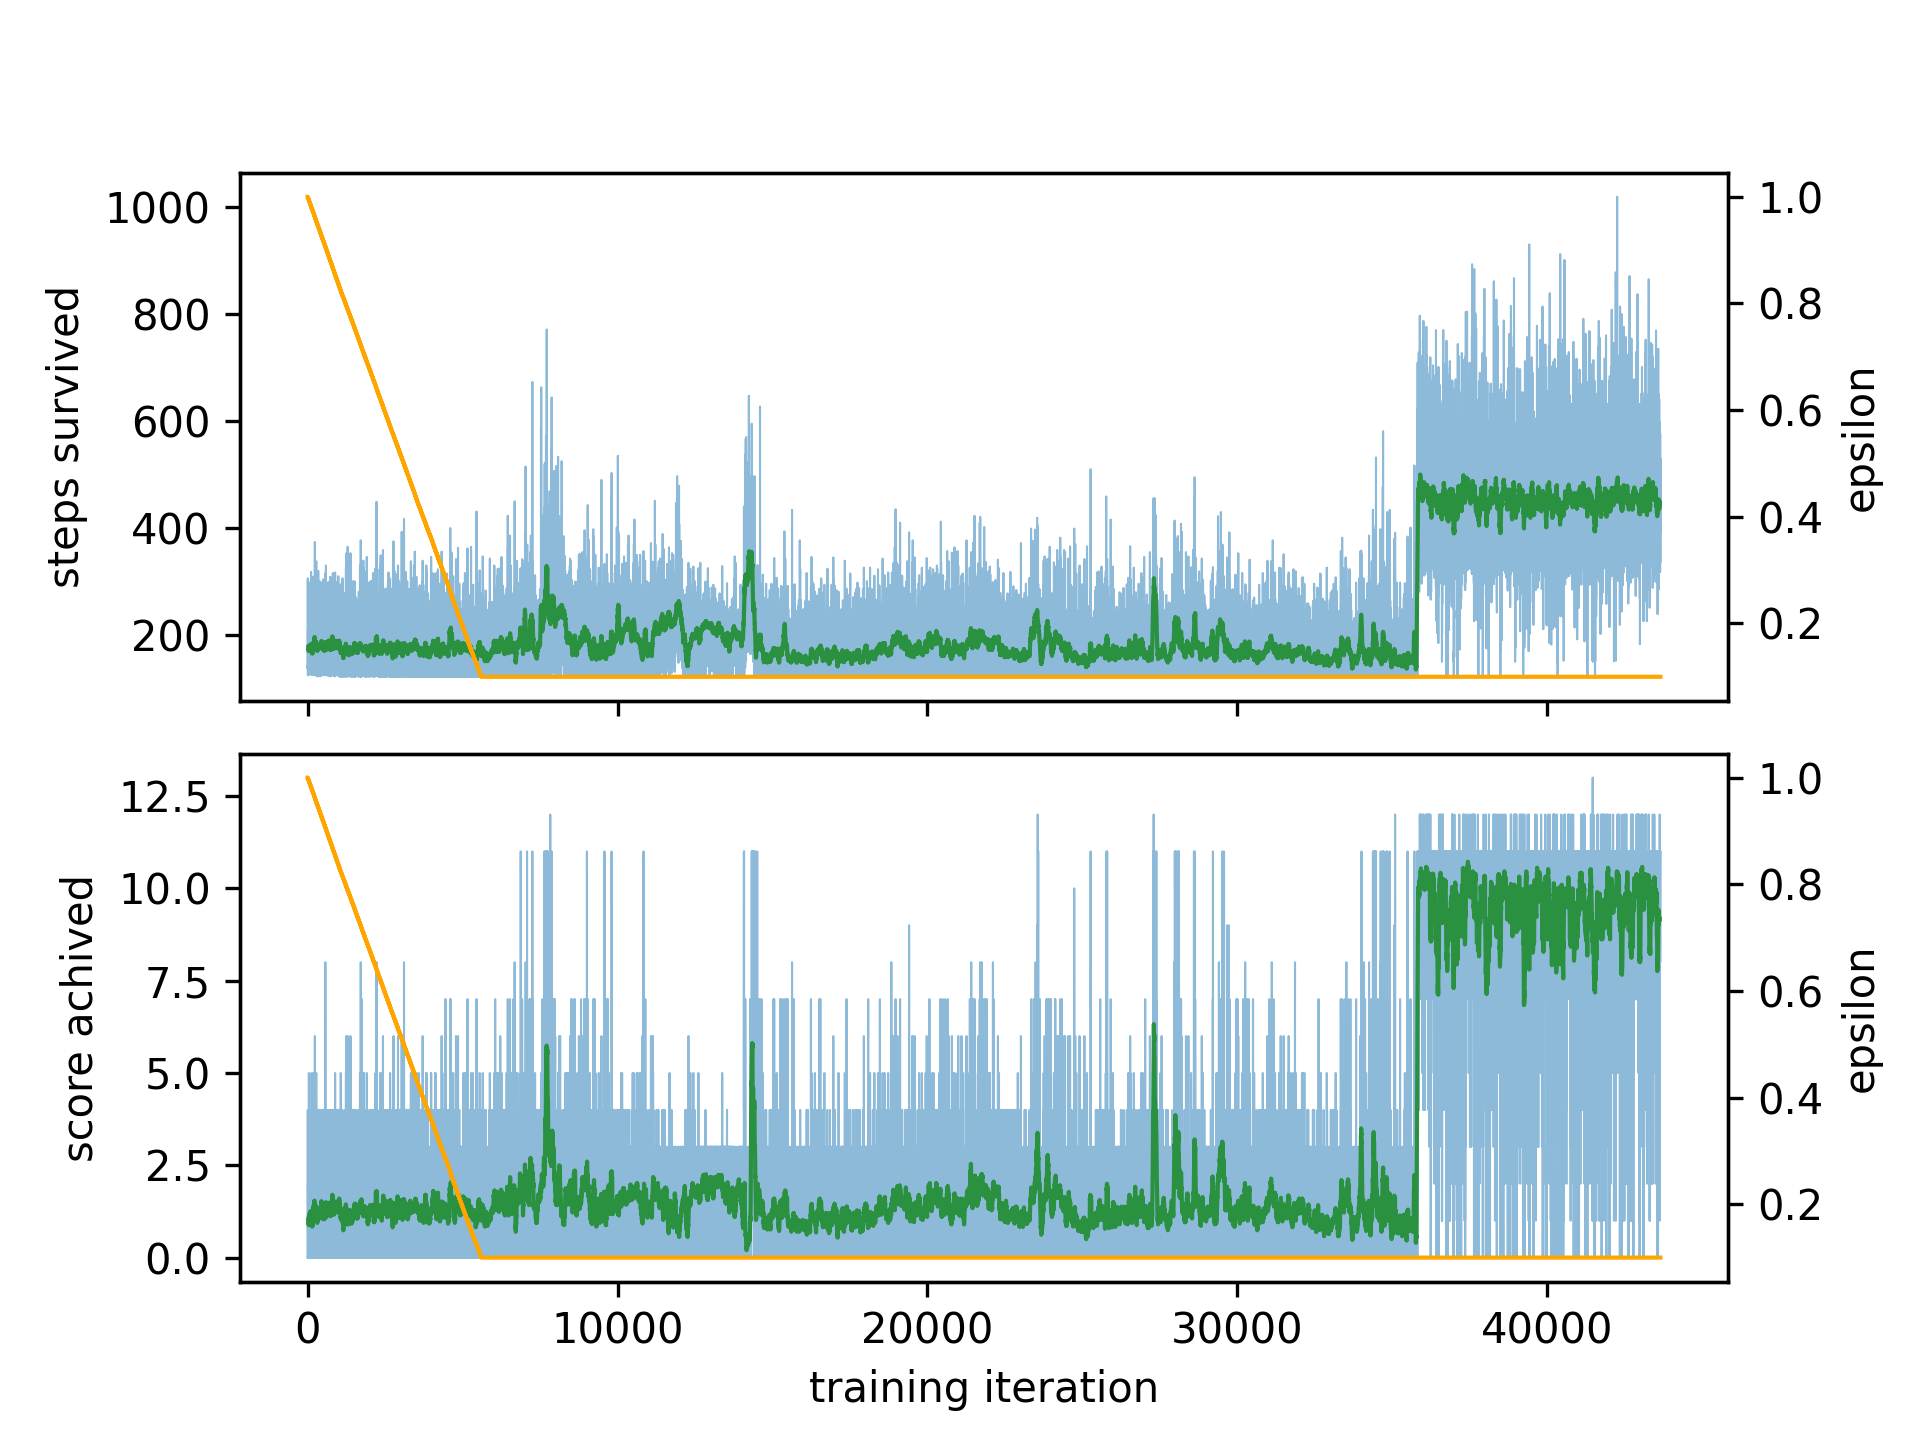
\includegraphics{breakout_10m}
    \caption{The performance of the agent when trained for 10 million steps. In orange the value of epsilon, in blue the steps per game for the top plot and score achived in the bottom plot. In green the moving average over the blue lines. For a closer look at the jump in performance around game $36000$ see \autoref{fig:breakout_10m_zoomed}}
    \label{fig:breakout_10m}
\end{figure}

From the moving average (green) we clearly see the agent had two early peaks where it seemd to grasp the game for a short while before collapsing again. Looking closer at the later jump (\autoref{fig:breakout_10m_zoomed}) note the improvement is quite a sudden, within 20 games the agent has grasped the basics of the game and is far outperforming its previous self only failing incidentilly. However we also see that save for one a single peak the agent never exceeds a score of 12.

\begin{figure}
    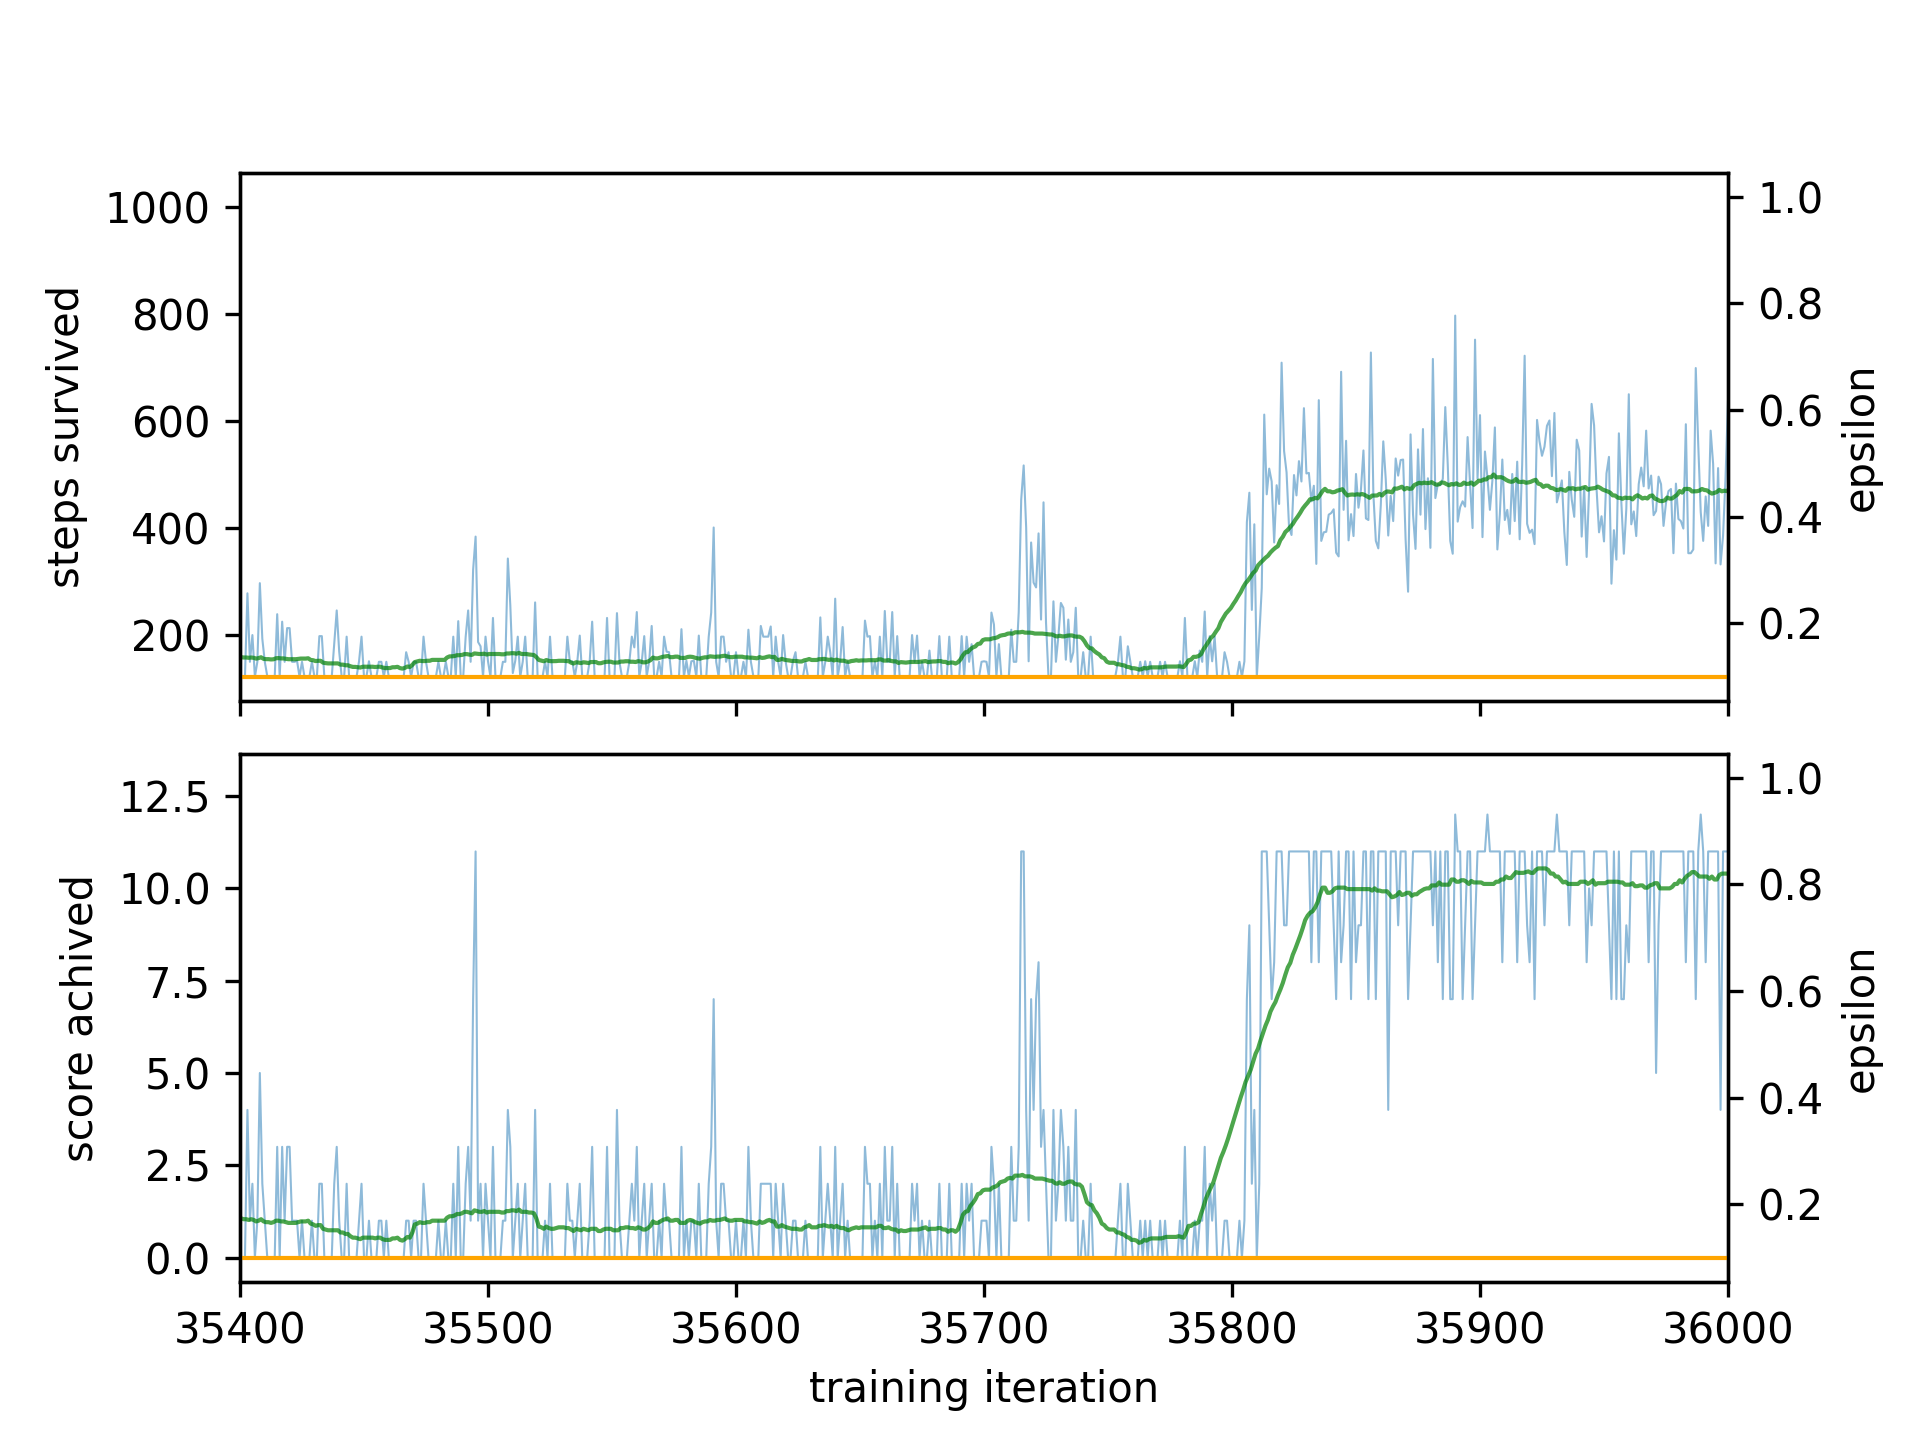
\includegraphics{breakout_10m_zoomed}
    \caption{The performance of the agent when it jumps up in performance at around game $36000$. In orange the value of epsilon, in blue the steps per game for the top plot and score achived in the bottom plot. In green the moving average over the blue lines.}
    \label{fig:breakout_10m_zoomed}
\end{figure}
